\documentclass[conference]{IEEEtran}
\usepackage{cite}
\usepackage{amsmath,amssymb,amsfonts}
\usepackage{algorithmic}
\usepackage{graphicx}
\usepackage{textcomp}
\usepackage{listings}
\usepackage{xcolor}

\begin{document}

\title{Rendering Water Using Compute Shaders and Navier Stokes Equations}

\author{\IEEEauthorblockN{Ivan Krukov}
\IEEEauthorblockA{\textit{Department of Computer Science}\\
\textit{Colorado School of Mines} \\
Golden, Colorado\\
ikrukov [at] mines.edu}
} \\

\maketitle

\begin{abstract}
	One area of particular interest within the field of games and fluid simulators is the ability to physically model properties of fluids such as water.
	Utilizing Navier Stokes Equations -- which can be used to describe incompressible, homogeneous fluids in an iterative fashion -- allows video game and simulation designers to encode realistic fluid interactions more effectively than traditional function based approaches such as Gerstner Waves. Such approaches are highly extendable to the rendering of different fluids such as fire, smoke, and volumes of water.
	This project is primarily centered around utilizing Navier Stokes Equations and a level set to realistically render a flowing river. Calculations for updating quantities in the fluid are performed in an OpenGL Compute Shader -- different from the traditional approach of implementing these calculations within the traditional rendering pipeline as a pixel or fragment shader. A vertex deformation shader is then used alongside a physically based lighting model to create a visually appealing and realistic looking river slice that was able to be rendered in real time.
\end{abstract}

\begin{IEEEkeywords}
Navier Stokes, Fluid Simulation, Physically Based Rendering, Vertex Deformation, Raytracing
\end{IEEEkeywords}

\section{Introduction}

This project primarily looked at the process of rendering water in OpenGL with the help of Navier Stokes Equations to physically model the geometry and velocity of the liquid along with Physically Based Rendering to produce realistic lighting effects. This technique of fluid simulation is important because it allows for highly realistic water modeling with the ability for easy extensions to user interaction (i.e allowing a user to pull their hand through water, a character jumping into a pool, etc). This can be accomplished by simply encoding interactions as a set of dynamic forces which is more difficult to do with other water rendering methods. Having a working implementation of the Navier Stokes Equations also gives way to relatively simple extensions to the modeling of different fluids such as smoke, clouds, and fire using the same shaders.

The brunt of the difficulty of implementing this project mainly came in the form of translating the Navier Stokes Equations into a form that can be computed on computer hardware. These equations have to be discretized and transformed into an iterative form in order to be able to simulate the evolution of a fluid over time. Alongside understanding the mathematical simplifications and assumptions that can be applied to Navier Stokes, additional thought has to go into actually rendering the fluid since Navier Stokes only describe how the velocity of the fluid behaves.

This paper will begin by looking at a series of related works in fluid/water simulation that influenced this project's implementation in \textit{Related Works}. With the basis of related work, implementation challenges of fluid rendering as well as solutions that this implementation explores will then be discussed in \textit{Problem Statement} and \textit{Problem Solution} respectively. Finally, the \textit{Results} section details the visual and performance results of this implementation.

\section{Related Work}

\subsection{Gerstner Wave Functions}

One approach to modeling behavior such as a ocean currents has to do with the physically modeling these behaviors with a combination of sinusoidal functions and calculating the height of a particular point of the fluid using a time variable. Specifically, \textit{Finch}\cite{gerstner} describes GPU water rendering techniques using the Gerstner wave function, defined by the equation:

\begin{figure}[htbp]
\centerline{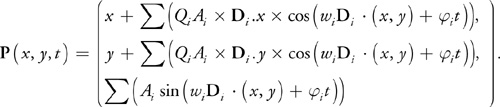
\includegraphics[width=0.5\textwidth]{gerstner.jpg}}
\end{figure}

Parameters such as amplitude ($A_i$), wave steepness ($Q_i$), and speed ($\phi$) can be controlled to change how the water's geometry behaves. These parameters could also be tuned to represent bodies of water other than oceans such as rivers and lakes. 

While Gerstner wave functions create relatively realistic ocean surfaces and could in theory be extended to different bodies of water, it is difficult to physically encode dynamic interactions with the fluid and different wave functions have to be considered if we want our fluid to behave differently.

\subsection{Ocean Lighting}

\textit{Bruneton, Neyret, and Holzschuch} looked into approaches in realistically lighting the surface of the ocean\cite{otherpbr}. Their approach consisted of multiple lighting passes to add refracted light, sky reflection, and sun reflection. Their work also expanded on approaches to applying physically based rendering models to water by identified that the Ross BRDF model would be best in representing the roughness of the ocean from all viewing scales. This is due to the fact that waves generated by a Gerstner wave train follow a Gaussian distribution of heights and with the application of traditional BRDF models such as Torrance Sparrow, the normals appear too uniform and improperly scaled for variations in the ocean's waves. The usage of a Ross BRDF also led to visual results that were similar to sample images used for rendering scenes.

Unfortunately due to time constraints, there wasn't enough time to implement the Ross or Ward BRDF in this implementation's lighting model.

\subsection{Fast Fluid Dynamics in Pixel Shaders}

\textit{Harris} provides much of the basis for understanding how one would implement Navier Stokes Equations on the GPU\cite{navierstokes}. This article primarily looks at a high level approach to using a incompressible, homogeneous fluid form of Navier Stokes -- modeling fluids that contain constant volumes within subregions over time and constant densities over space and time. Harris also does most of the work in approximating the gradient, laplacian, and divergence operators used in the original Navier Stokes equations to a discrete and iterative form that can be programmed on a GPU.

In terms of GPU implementation details, Harris' approach used multiple 2D texture units to store quantities such as velocity and dye color and iteratively updated these quantities every draw cycle with multiple Direct3D pixel shaders. Implementation details and understandings of the terms involved in Navier Stokes are discussed further in the section \textit{Problem Solution}.

\subsection{Ray marching Approach to Rendering Fluid Volumes}

While \textit{Harris} looked at the implementation of fluid dynamics on the GPU, few details were expressed on how to render the fluid that was being modeled. \textit{Crane, Llamas, and Tariq} expanded on this by outlining an approach on rendering multiple different 3D fluids in the form of smoke, water, and fire\cite{fluidrender}. Specifically in the context of water, this article suggests expanding on \textit{Harris} by using a 3D version of the Navier Stokes equations with 3D textures.

In addition to having a 3D texture for velocity, the article also introduced the usage of a level set to represent a fluid volume that can be updated using the advection routine of a Navier Stokes shader. The level set -- commonly used to model water surfaces -- is a set of scalar values representing:

\begin{itemize}
	\item $x > 0$: Cells that contain air

	\item $x < 0$: Cells that contain water

	\item $x = 0$: The exact point the water's surface is encountered

\end{itemize}

Additional optimizations were also realized with the ability to mask computations based on cells that contained air. This is due to the fact that pressure computations can be skipped in these cells(we don't care about the pressure of the air to model a fluid) and the application of external forces (we mainly care about forces when directly applied to the fluid).

With this 3D level set texture, the authors then outline that the front faces of a bounding box of the fluid needs to be rendered. Rays are then cast into this bounding box that generates a separate texture that keeps track of the entry point of a ray and the depth that the ray traverses through the volume before encountering another front face (i.e of a different object in the scene) or the end of the bounding box. This ray data is then used in a separate quad shader that dictates how a 3D texture representing the volume is sampled. In the case of water, this texture is the level set discussed earlier. Once a level set value of 0 is encountered, the shading routine for the water's surface is then run. Figure~\ref{volumerender} represents this concept at a high level for the rendering of smoke.

\begin{figure}[htbp]
\centerline{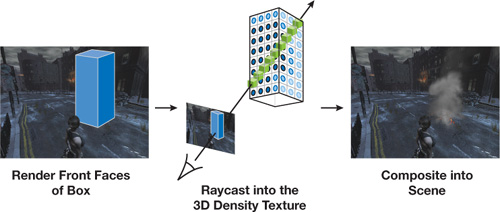
\includegraphics[width=0.5\textwidth]{volumerender.jpg}}
\caption{Ray Tracing Rendering Process for 3D fluids \cite{fluidrender}}
\label{volumerender}
\end{figure}

\section{Problem Statement}
Modelling water is inherently challenging in case when one would wish to be able to encode physical interactions or forces on the fluid. Approaches such as using functions to approximate wave heights such such as Gerstner Wave \mbox{Trains -- while} producing visually appealing results in real \mbox{time -- fall} short in how extensive the user can interact with the fluid. Modelling water with fluid dynamics can allow for the manipulation of a physical representation of the fluid with respect to velocity, giving way to being able to encode different bodies of water with different static forces as well as (if desired) dynamic forces such as user interaction. However, the brunt of the challenge in fluid simulation is being able to understand and translate fluid dynamics involving continuous calculus operations to something that can be computed on computer hardware.
While traditional approaches have been able to achieve real-time results and have gone through the approximation steps to run a discrete form of the Navier Stokes equations on the CPU/GPU, these approaches also came 5--10 years before compute shaders were introduced into the core of OpenGL in version 4.3. As such, much of the mathematical work that went into solving these equations was done in the form of a G-buffer like structure with the help of a fragment shader or Direct3D pixel shader. These approaches inherently perform some unnecessary computational steps such as processing and interpolating values for the points of a screen space quad, potentially sampling texture units more than necessary for updating a pixel in the simulation grid, and performing per-fragment operations before finally writing to the render buffer. Compute shaders can help reduce these redundant computations by giving more fine-grained control over how simulation values are updated.

In addition to the modelling challenges and potential improvements by transitioning to a compute shader, there are also additional factors not considered in the papers such as creating the illusion of a continuous fluid volume. This is particularly crucial for this implementation since the segment of the river being rendered is inherently continuous. Considerations have to be made on how to exactly initialize the level set and set boundary conditions that produce visually appealing behaviour.

\section{Problem Solution}

The following section details the technical implementation details of the final codebase. Much of the following work is based on prior works with the exception of applying Navier Stokes computations on the GPU alongside implementation hacks such as treating the level set as a height map to avoid ray tracing and modifications to the level set to create the appearance of a continuous volume.

\subsection{Navier Stokes GPU Approximations}

Much of the mathematical work is attributed to the work done by \textit{Harris} from the \textit{Related Works} section. In general, the Navier Stokes Equation for homogeneous, incompressible fluids can be expressed as:

\begin{equation}
	\frac{\partial \mathbf{u}}{\partial t}=-(\mathbf{u} \cdot \nabla) \mathbf{u}-\frac{1}{\rho} \nabla p+\nu \nabla^{2} \mathbf{u}+\mathbf{F}
\end{equation}

This can be thought of as the combination of multiple acceleration terms dictating the evolution of a fluid's velocity, $u$, over time. The updated velocity of the fluid can then be used to update other quantities within the fluid that dictate how it the fluid appears.

Within the final implementation, each acceleration term ends up being consolidated and processed within its own compute shader. Certain approximations to calculus operators such as Jacobi Iteration for the laplacian are also contained within their own shader (calculus.c.glsl). The following paragraphs go into more detail what each of the acceleration terms in the equation are alongside how these quantities are approximated discretely.

\paragraph{Advection $(-(\mathbf{u} \cdot \nabla) \mathbf{u})$} Advection at a high level encodes the fact that velocity can move quantities within a fluid such as dye colors, the level set, and even velocity itself. As such, advection could instead be expressed of in terms of updating the position of a particle using Euler's forward integration method rather than in terms of the divergence operator:

\begin{equation}
\mathbf{r}(t+\delta t)=\mathbf{r}(t)+\mathbf{u}(t) \delta t
\end{equation} 

One principle concern with this approach is that if $\mathbf{u}(t) \delta t$ gets larger than the size of a grid cell (especially in the case of large time steps), the calculation becomes unstable. Therefore, the final implementation uses an implicict method of integration which can be visualized by Figure~\ref{advection}.

\begin{equation}
q(\mathbf{x}, t+\delta t)=q(\mathbf{x}-\mathbf{u}(\mathbf{x}, t) \delta t, t)
\end{equation}

	This method effectively states that the quantity at a point x at time $t + \delta t$ is calculated by getting quantity at point $\mathbf{x} - \mathbf{u}$ at time $t$ , where $\mathbf{u}$ is the velocity at our current position and time. Since the resolution of our grid isn't infinite, it is often the case that this projection backwards doesn't perfectly align with the sampling grid.
Thus, the four points surrounding the traced point are bilinearly interpolated to approximate the quantity that would have been at that point. This is most easily accomplised with rectangular texture units, which are used in the final implementation.
This is due to the fact that one could then sample a texture based on a texture's dimensions(whole numbers) and use the fractional portion of a traced coordinate for mixing proportions. Flooring and ceiling functions could then be used to access the nearest points in the grid. 

Another customary modification to the advection term is to multiply a dissipation constant to the advected quantity to represent behavior such as the fading of dye through a fluid, usually taking a value very close to 1 (e.g $0.99$). This method is applied to the final implementation with the visual result of the modeled river sloping slightly downards along with the settling of the fluid when no forces are applied.

The process described for the implicit method of forward integration with dissipation is encoded and performed in the shader advect.c.glsl, with the OpenGL calls to orchestrate the execution of this routine found in the C++ function advect(timeStep).


\begin{figure}[htbp]
\centerline{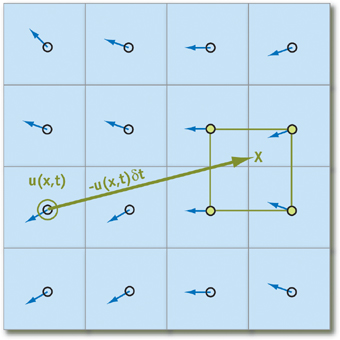
\includegraphics[width=0.35\textwidth]{advection.jpg}}
\caption{Tracing the Velocity of a Particle for Stable Advection\cite{navierstokes}}
\label{advection}
\end{figure}

\paragraph{Pressure $(-\frac{1}{\rho} \nabla p)$} The pressure term primarily encodes Newton's Second Law, where pressure can often build up in a fluid due to the squishing of fluid particles. This squishing of particles imparts an acceleration of its own onto the fluid. The magnitude of this effect is tunable through changing the fluid's density $\rho$. However, one major factor in determining the effect of pressure is to solve for the actual pressure field since velocity and fluid quantities are the only variables that are being tracked.

In order to get to a point where one could solve for the pressure term, some groundwork has to be built up. Considering the constraint placed on the modeled fluid being homogeneous and incompressible, this tells us that the divergence of the resulting velocity field needs to be zero at each time step. Luckily, just like how vectors can be broken into $\hat{i}$ and $\hat{j}$ components, so too could vector fields be broken up into divergence and divergence free fields of the form:

\begin{equation}
	\mathbf{w}=\mathbf{u}+\nabla p
\end{equation}

Where w is a vector field in the region of fluid that is being modeled, u has a divergence of 0 parallel to the region of fluid, and p is a scalar field (in this case, pressure). Formally, this technique is called the Helmholtz-Hodge Decomposition, and it allows us to express the pressure term as a subtraction of a pressure gradient (Equation~\eqref{pressuregrad}) and solve for the pressure field by applying the divergence operator on both sides of the Helmholtz-Hodge Decomposition to solve for pressure(Equation~\eqref{pressuresolve}).

\begin{equation}
	\mathbf{u}=\mathbf{w}-\nabla p
\label{pressuregrad}
\end{equation}


\begin{equation}
	\nabla \cdot \mathbf{w}=\nabla \cdot(\mathbf{u}+\nabla p)=\nabla \cdot \mathbf{u}+\nabla^{2} p
	\label{pressuresolve}
\end{equation}

Since the divergence of velocity is zero from our fluid constraints, Equation~\eqref{pressuresolve} could be simplified into the Poisson Equation described in Equation~\eqref{pressuresolvenodiv}. This form has solver techniques that can be now implemented on computer hardware, discussed further in \textit{Solving the Poisson Equation}

\begin{equation}
\nabla^{2} p=\nabla \cdot \mathbf{w}
\label{pressuresolvenodiv}
\end{equation}


Implementation-wise, Pressure is solved using routines in calculus.c.glsl for calculating the divergence of velocity along with iteratively solving for the pressure gradient with the divergence of velocity using Jacobi iteration described in \textit{Solving the Poisson Equation}.


\paragraph{Viscous Diffusion $(\nu \nabla^{2} \mathbf{u})$} Viscous diffusion allows for the modeling of fluids of varying consistencies and thicknesses. This allows us to encode different fluid behavior when dealing with a fluid such as water versus maple syrup. In essence, this term acts as a resistance to flow that causes a diffusion of momentum(hence the term Viscous Diffusion). 

In a very similar way to advection, Viscous Diffusion can also be expressed in discrete terms by the equation:

\begin{equation}
	\label{diffunstable}
\mathbf{u}(\mathbf{x}, t+\delta t)=\mathbf{u}(\mathbf{x}, t)+\nu \delta t \nabla^{2} \mathbf{u}(\mathbf{x}, t)
\end{equation}

Where $\nabla^2$ is the discrete form of the Laplacian Operator:

\begin{equation}
\nabla^{2} p=\frac{p_{i+1, j}+p_{i-1, j}+p_{i, j+1}+p_{i, j-1}-4 p_{i, j}}{(\delta x)^{2}}
\end{equation}

Just like how advection experienced stability issues with large timesteps, so too does the diffusion term in Equation~\eqref{diffunstable}. This is also resolved by using an implicit method of integration to get to a form that can then be solved with a Poisson equation solver: 

\begin{equation}
\left(\mathbf{I}-\nu \delta t \nabla^{2}\right) \mathbf{u}(\mathbf{x}, t+\delta t)=\mathbf{u}(\mathbf{x}, t)
\end{equation}


Implementation-wise, Viscous Diffusion is solved through iterative calls to Jacobi iteration in the C++ function diffuse(timeDelta), which then is responsible for dispatching multiple compute shader runs in calculus.c.glsl.

\paragraph{Solving the Poisson Equation} Since Pressure and Viscous Diffusion could be rewritten in the form of Poisson equations (linear algebra matrix equations in the form $Ax=b$, solver techniques for these equations could be implemented on the GPU to get these quantities. This is accomplished with the usage of a technique called Jacobi iteration to iteratively approach the solution for these quantities. The general form for Jacobi iteration -- derived from the discrete form of the Laplacian Operator -- is described by the equation: 

\begin{equation}
x_{i, j}^{(k+1)}=\frac{x_{i-1, j}^{(k)}+x_{i+1, j}^{(k)}+x_{i, j-1}^{(k)}+x_{i, j+1}^{(k)}+\alpha b_{i, j}}{\beta}
\end{equation} 

For good convergence on the solution and high resolution results, 20--50 iterations and 40--80 iterations are recommended for Viscous Diffusion and Pressure respectively\cite{navierstokes}. The final implementation opts to use 30 iterations for both effects. Table~1 outlines what each parameter is set to when solving the Laplacian for Viscous Diffusion and Pressure. $\delta x$ represents the scale of our grid ($1$ since there is one cell per pixel) and $\delta t$ represents the time step. x and b represent the texture units(and image unit for storing $x^{(k+1)}_{i,j}$ ) that would be bound on the execution of the Jacobi iteration shader. The pressure computation also relies on the computation of the divergence of velocity which is performed by a separate shader routine and stored in a texture unit prior to pressure calculations. The overall routine to perform Jacobi Iteration along with other calculus operators are stored in the shader calculus.c.glsl.

\begin{table}[htbp]
\caption{Jacobi Iteration Parameters for Solving Laplacian Operators}
\begin{center}

	\begin{tabular}{|c|c|c|c|c|}\hline
		Property & $\alpha$  & $\beta$  & $\mathbf{x}$  & \mathbf{b} \\\hline
		Diffusion & $\frac{(\delta \mathbf{x})^2}{\nu\delta t}$ & $4 + \alpha$ & velocity  & velocity \\\hline
		Pressure & $-(\delta \mathbf{x})^2$  & 4 & pressure & $\nabla \cdot \mathbf{v}$  \\\hline
	\end{tabular}
\label{termdesc}
\end{center}
\end{table}

\paragraph{External Forces $(\mathbf{F})$} The external forces term simply encodes any forces (static, constant forces such as gravity or dynamic forces such as wind or user interaction) that impart an acceleration or impulse that changes the velocity of the fluid. This term is the most straightforward of them all since it doesn't involve any complex calculus and is a simple addition based on time.

In terms of the implementation, the addition of external force is performed by a separate shader called force.c.glsl. This shader has multiple subroutines which can be switched between to change the force being applied to the fluid domain using the "C" key when the text on the top of the screen says that the user is in "force mode" (toggled using the "F" key). This shader implements four force models to play around with different fluid dynamics defined by simple equations:

\begin{itemize}
	\item \textbf{River} applies a constant force based on a passed in uniform vec4 "force". This is the default mode of operation with a force vector representing the pull of a river(constant, to the lower left portion of the fluid texture unit).

	\item \textbf{Whirlpool} plays around with moving the fluid in a slightly circular pattern around the center of the fluid.

	\item \textbf{Ripple} involves a force that increases as you move radially away from the center of the fluid.

	\item \textbf{Inward} acts as the opposite of ripple and pulls all quantities inwards.

	\item \textbf{Nochange} sets force to zero.
	
\end{itemize}

\paragraph{Boundary Conditions} In order to properly pose the mathematical approximations described for the Navier Stokes equations detailed above, boundary conditions have to be enforced for the grid. These come in the form of a no-slip condition for velocity, stating that $u \to 0$ as we approach the bounds of our grid along with a constraint required for the Poisson pressure equation called a pure Neumann boundary condition, where the change in pressure relative to the direction normal of a boundary is zero (In other words, $\delta p / \delta n = 0$). 

In terms of shader implementation, both of these constraints can be simply solved for by enforcing that the values directly at the edge of the boundary are zero. However, due to the fact that the samples in our grid represent the middle of a cell, we have to instead take the two adjacent cells to a border and solve for the border pixel value where their average would be zero. This can be visualized with Figure~\ref{boundaryconditions} which outlines the offsets from the border that would be used to solve for the average of zero, with the result being stored in the shaded cells.

\begin{figure}[htbp]
\centerline{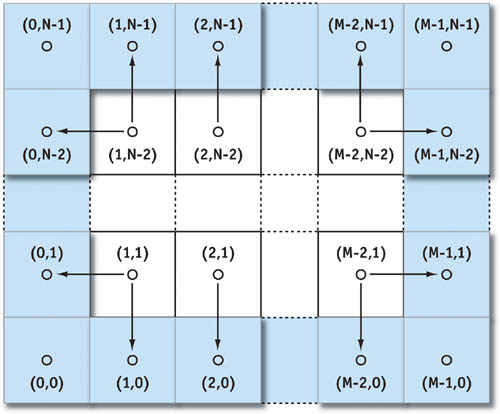
\includegraphics[width=0.37\textwidth]{boundaries.jpg}}
\caption{Sampling Cell Centers for Boundary Condition Enforcement\cite{navierstokes}}
\label{boundaryconditions}
\end{figure}

Traditionally, the implementation described by \textit{Harris} involved masking computations to be explicitly on the boundary by having a rendering pass which draws line primitives on the edges of a quad (the quad being used for Navier Stokes computations). Since this approach uses compute shaders, this masking of computations is instead a different workgroup scheduling further described in the section on Compute Shader Applications. All of the boundary condition calculations are performed with the routine defined in boundary.c.glsl.

\subsection{Compute Shader Application}

While traditional implementations looked at fragment and pixel shader approaches for running Navier Stokes computations on textures, this approach looked more at the usage of compute shaders to improve computational performance. Most of the shaders described above for performing a step of the iterative Navier Stokes Computations were compiled as programs with a single compute shader. These compute shaders typically take in a number of sampler2DRect texture units for velocity, pressure, and the level set (in the case of advection) depending on the Navier Stokes step that is being performed. All of the compute shaders also take in an image2DRect texture unit which is used so the compute shaders can do meaningful work and store their result in a place that can be accessible for future computations and draw calls. The process of loading specific uniforms and texture units is described by the parameters in previous sections as well as the C++ functions named after each Navier Stokes Operation (advect, diffuse, projection (pressure), boundary, applyForce)

In terms of work group allocation, all of these compute shader programs with the exception of the boundary program operated with TEXDIM by TEXDIM global work groups. Each work group in an invocation was responsible for updating exactly one pixel in the resulting image2D using the imageStore GLSL command. In the case of the boundary conditions program, there are instead TEXDIM by $1$ global workgroups and a local size of $4$ local workgroups. The local workgroup ID is used to effectively index the top, bottom, left, and right sides of the image. This leads to a structure where there are 4 image writes per global work group invocation for the ith pixel on the top, bottom, left, and right boundaries of the image.

In addition to the aforementioned compute shaders for performing Navier Stokes computations, an additional compute shader is used for calculating the bump map of the level set. The reason for this operation is described in more detail in the next section outlining the fluid rendering process. The code for this routine is defined in normals.c.glsl.

Due to the memory model of OpenGL, undefined behaviour may occur when performing concurrent reads and writes to the same texture unit or SSBO on a compute shader pass. As such, pairs of rectangular texture units are used for velocity, pressure, and the level set. In events where a velocity texture unit needs to be read and written to concurrently (e.g in the case of velocity advecting itself), one unit is bound as a write-only image2DRect while the other is bound as a standard sampler2DRect. A consistent access pattern to these textures is maintained to make sure the latest texture representation is being read while stale values are overwritten. This is primarily accomplished with the help of a user-defined function called swapAndBindTexUnits which is responsible for swapping the texture that is being read/written and binding them to the corresponding sampler/image binding points for the next shader call. In places where a shader invocation only needs to read the latest updated value of a texture unit, swapAndBindTexUnits guarantees that the second texture unit (e.g velocityTextures[1]) contains the desired value.


\subsection{Fluid Rendering Process}
Instead of performing a ray tracing approach to rendering 3D water as described in the \textit{Related Works}, this implementation instead opts for a simpler approximation of the water's surface by using the level set as a height map. The level set texture is processed by a separate compute shader called normals.c.glsl. This routine is responsible for writing out a bump map texture which stores the original position of the particle alongside the normal based on the gradient using the surrounding level set values. The bump map is then used as an input for rendering in the vertex deformation shader and PBR fragment shader.

At a high level, the OpenGL rendering process for each pixel involves the following steps:

\begin{enumerate}
	\item Compute the timedelta

	\item Perform advection, diffusion, force application, pressure, and boundary condition evaluation on the velocity texture

	\item Use the updated velocity to advect the level set

	\item If the continuous level set hack is being used (toggled by pressing "S"), use the boundary program to set the level set at the edge of the texture unit

	\item Calculate the bump map (normals with position) for the level set(treated as a height map)

	\item If we are rendering in quad debug mode (toggled by pressing "D"), render a screenspace quad showing textures such as the velocity, level set, and pressure field.

	\item If we aren't in debug mode, render the skybox

	\item Render the water using the bump map, skybox cube map for reflections, and uniform parameters for water fluid material and lights. This is done with triangle strips or line strips if the user has cheap wireframing enabled (toggled by pressing "W")

\end{enumerate}

In addition to the rendering process and key controls mentioned above, the user can also reinitialize the level set texture by pressing the "R" key.

Due to time constraints, there wasn't ample time to implement the Ross model of physically based rendering of the water's surface. The Torrance Sparrow model is used instead with a material that has a roughness of $0.23$, non-metallic, and a grayish blue color. There weren't many good sources on good values for modelling water, so these values were achieved by tweaking parameters until a good visual result was achieved. 



\section{Results}

Figure~\ref{fluidrender} shows the visual results of applying the aforementioned rendering techniques to a fluid using the river force application. Figure~\ref{levelsetrender} shows the corresponding texture debug view of the level set currently being drawn. This render specifically utilized random initialization of the level set for simulation initial conditions, random reinitialization of the level set which can be observed on the top/right edges of the rendering, and a constant static force that influences velocity to pull the particles to the bottom left of the rendered volume. In motion, this results in a convincing look to the river and even cause small scale distortions/shimmers on the surface near specular highlights. The Whirlpool force application is also demonstrated in Figure~\ref{whirlrender}.

In terms of frame rate, the program averages at 21 frames per second using integrated graphics on an Intel Core I5 CPU, 300$\times$300 textures for storing simulation parameters, 30 Jacobi iterations for approximating the laplacian operators involved in the diffuse and pressure terms, and a vertex deformation mesh of around 115,000 triangles. With dedicated graphics hardware or a different algorithm for calculating the laplacian, the frame rate would likely be closer to 60 frames per second.

\begin{figure}[htbp]
\centerline{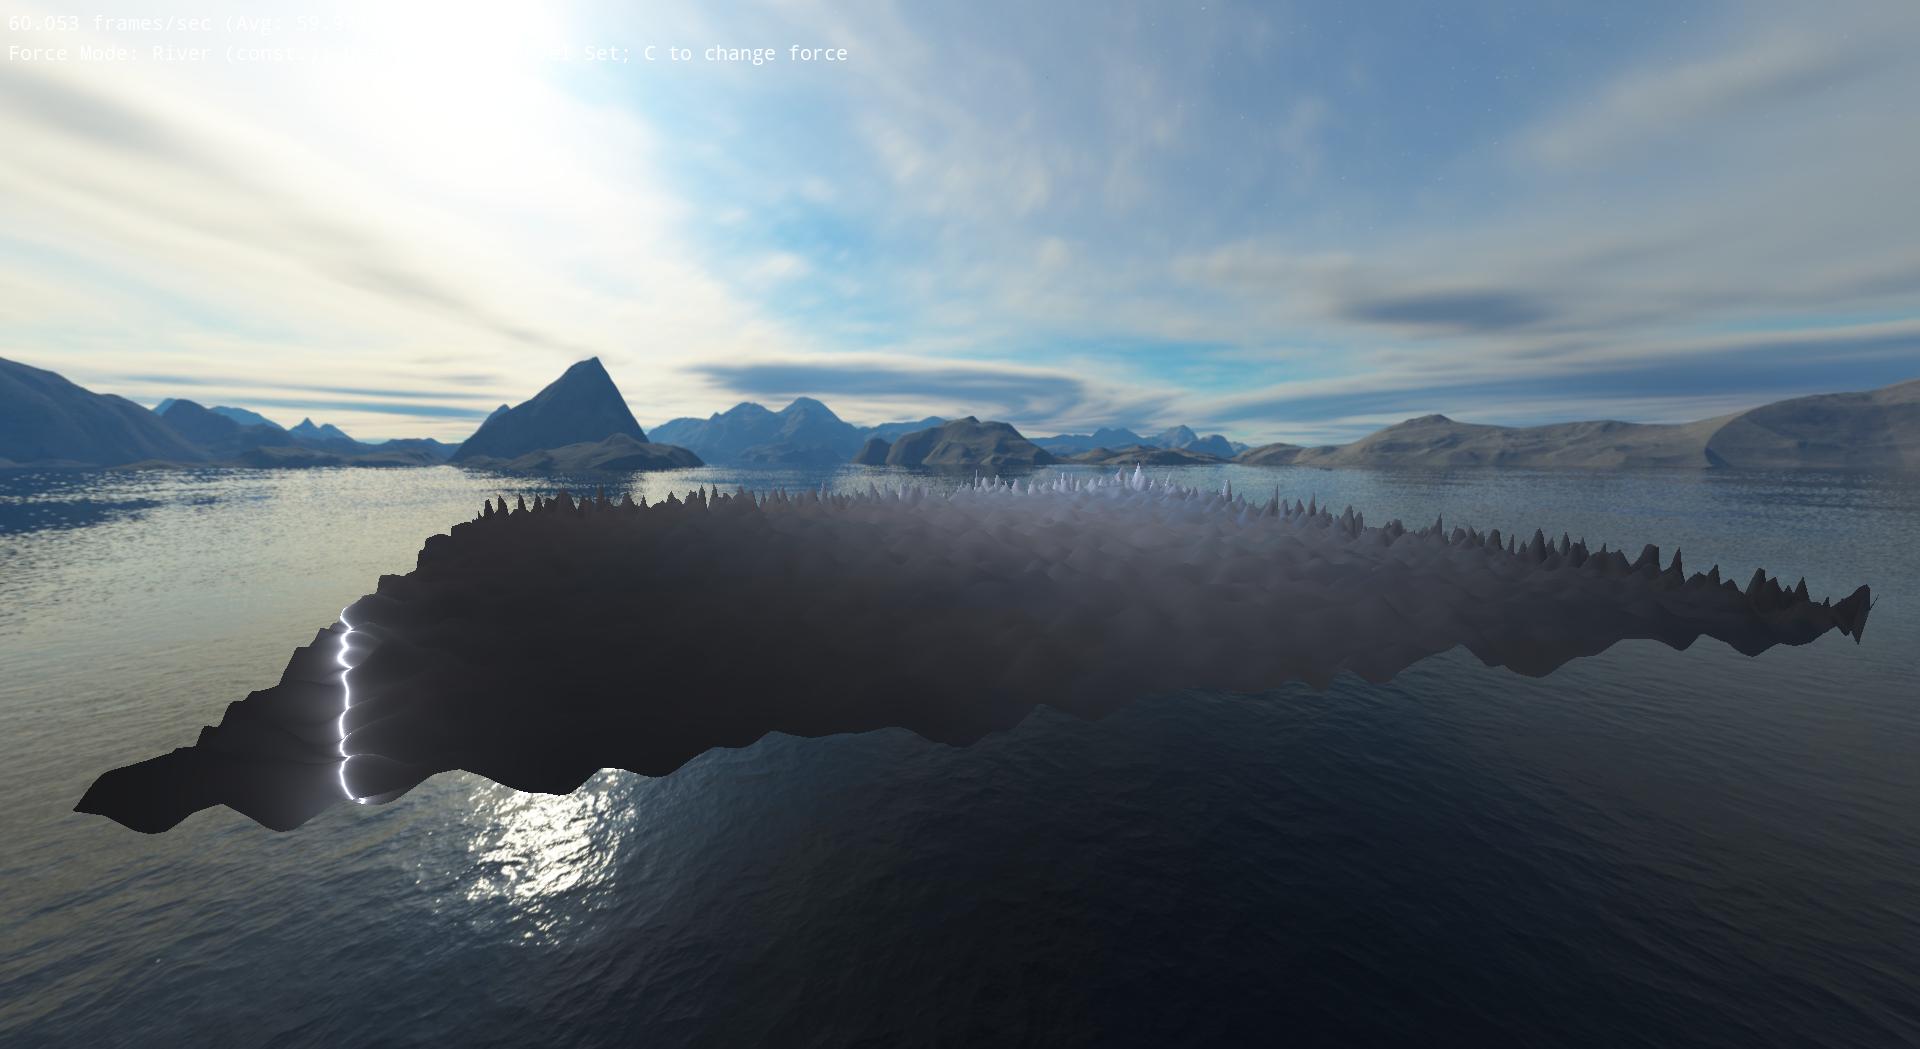
\includegraphics[width=0.5\textwidth]{waterrender.png}}
\caption{Final Rendered Result}
\label{fluidrender}
\end{figure}

\begin{figure}[htbp]
\centerline{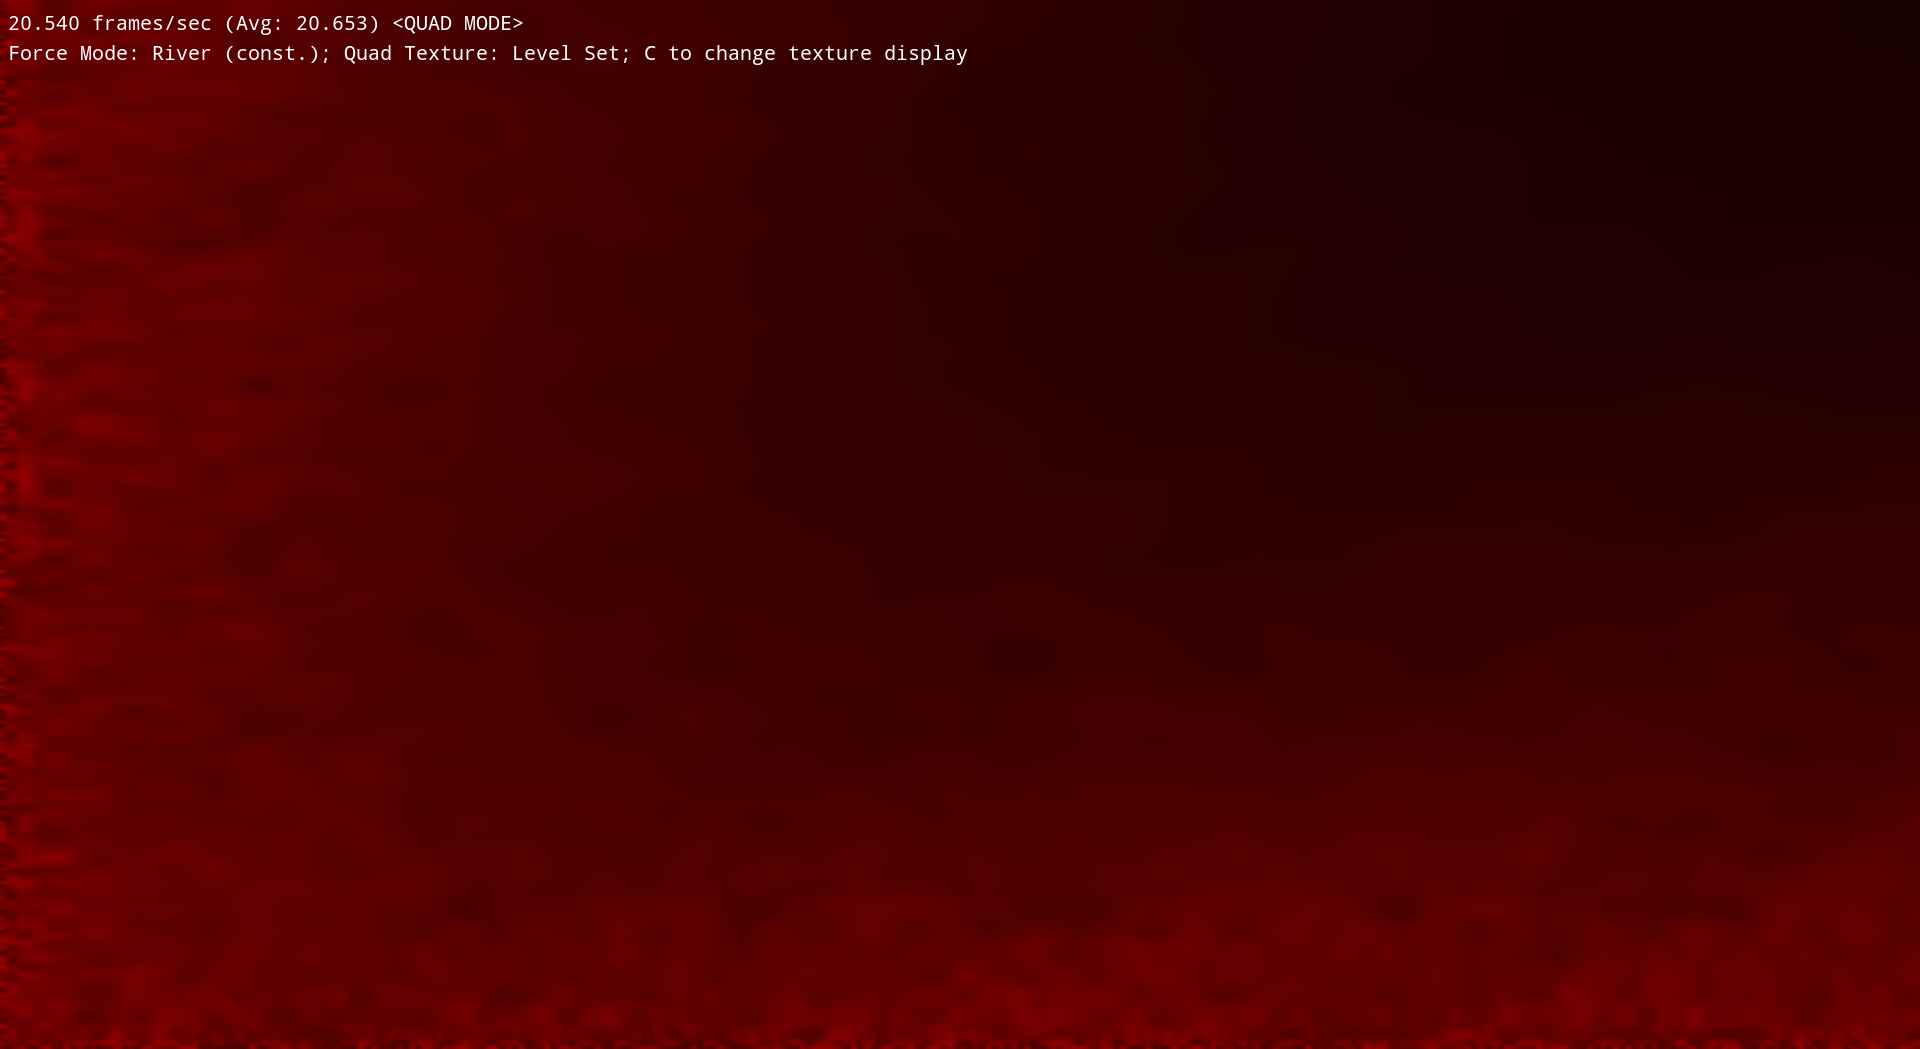
\includegraphics[width=0.5\textwidth]{levelset.png}}
\caption{Advected Level Set Quantity}
\label{levelsetrender}
\end{figure}

\begin{figure}[htbp]
\centerline{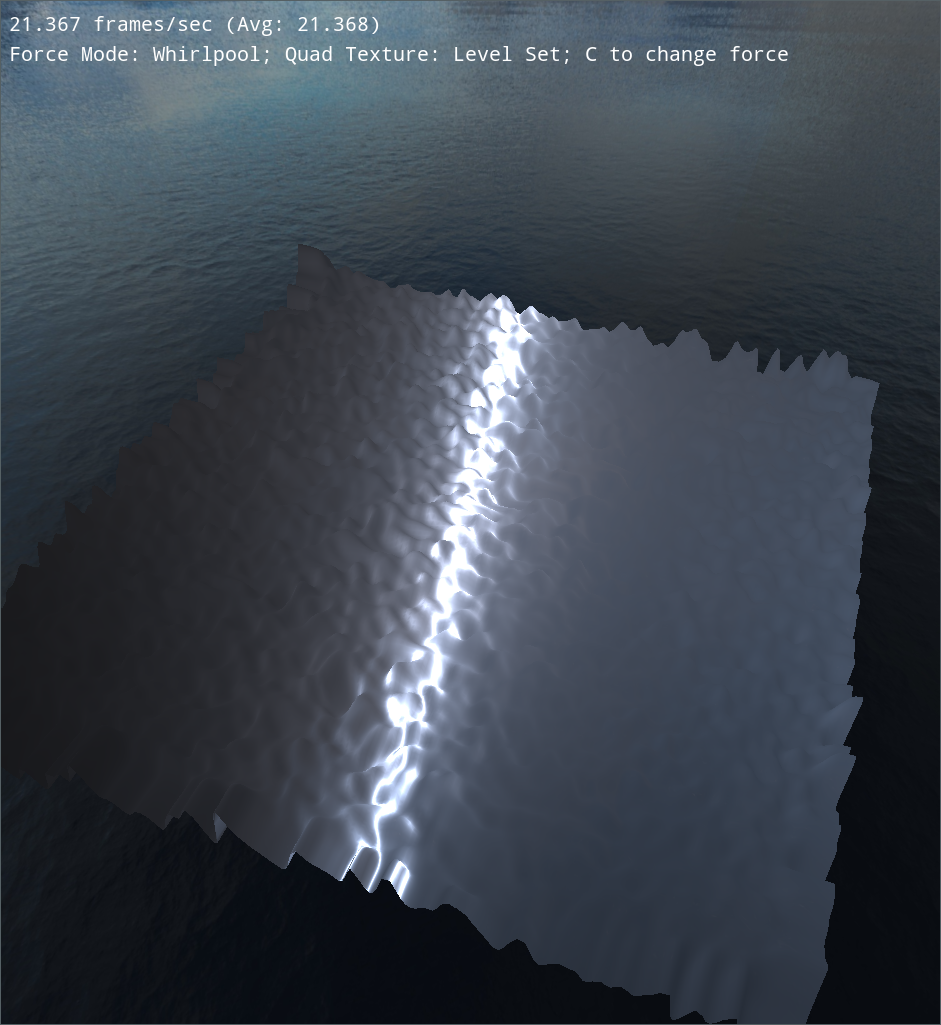
\includegraphics[width=0.5\textwidth]{whirl.png}}
\caption{Whirlpool force rendering}
\label{whirlrender}
\end{figure}

\section{Conclusion}

This project looked at the implementation of the Navier Stokes Equations in an OpenGL compute shader in order to render a realistic looking river. This is different from prior approaches which just look at using fragment/pixel shaders or that seek to approximate surface behaviour using wave trains. This project also simplified the modelling of the water's surface by looking at the level set as a height map that is advected and used for a vertex deformation shader. While there wasn't enough time in the semester to implement some of the lighting/texturing features (i.e adding sea foam), the visual results of the program are still look relatively impressive while maintaining a workable frame rate on low end graphics hardware.

This project served as a great opportunity to get a glimpse of how computer graphics programmers take math and physics heavy concepts and massage models into something that could be used by the GPU to improve the realism of a simulated effect. This project also served as a good learning experience for how to model fluids on the GPU and gives a good baseline of shaders that could be used in different projects for other fluids outside of water such as fire and smoke.

Future work for this implementation includes adding the ability for the user to impart impulses on the fluid, replacing the Jacobi Iteration algorithm with one that converges to a solution in fewer iterations, and the implementation of the Ross BRDF in order to be able to compare visual results. It would have also been interesting to create an implementation using only fragment shaders for Navier Stokes computations and see the magnitude of performance gains seen when using a compute shader over a fragment shader.

\begin{thebibliography}{00}

\bibitem{gerstner} M. Finch. ``Effective Water Simulation from Physical Models''. GPU Gems ch. 1, vol. 1. https://developer.nvidia.com/gpugems/gpugems/part-i-natural-effects/chapter-1-effective-water-simulation-physical-models. April 2004.

\bibitem{navierstokes} M. Harris, “Fast fluid dynamics simulation on the GPU,” ACM SIGGRAPH 2005 Courses, pp. 220-es, Jul. 2005. 

\bibitem{fluidrender} K. Crane, I. Llamas, and S. Tariq. ``Real-Time Simulation and Rendering of 3D Fluids''. GPU Gems ch. 30, vol. 3. https://developer.nvidia.com/gpugems/gpugems3/part-v-physics-simulation/chapter-30-real-time-simulation-and-rendering-3d-fluids. August 2007.

\bibitem{otherpbr} E. Bruneton, F. Neyret, and N. Holzschuch, “Real-time Realistic Ocean Lighting using Seamless Transitions from Geometry to BRDF,” Computer Graphics Forum, vol. 29, no. 2, pp. 487–496, Jan. 2010. 

\end{thebibliography}

\end{document}
